\ExerciseAppendix

\begin{enumerate}
\def\labelenumi{\arabic{enumi})}
\tightlist
\item
  Let X be a Hausdorff topological space on which there is defined an associative law of composition written multiplicatively. Generalize Definition 1 to the case of a family \((x_{i})_{i\in I}\) of elements of X, whose index set I is linearly ordered. For each finite subset J of I, let \(p_{J}\) denote the product \(\prod_{i\in J} x_{i}\) of the sequence \((x_{i})_{i\in J}\) .
\end{enumerate}

If X is a complete topological group, then a family \((x_{i})_{i\in\mathbf{I}}\) of points of X is multipliable if and only if, given any neighbourhood V of the identity element e of X, there exists a finite subset \(J_{0}\) of I such that, for every finite subset J of I containing \(J_{0}\) , we have \(p_{J}(p_{J_{0}})^{-1}\in V\) {[}or \((p_{J_{0}})^{-1}p_{J}\in V\) {]}.

\begin{enumerate}
\def\labelenumi{\arabic{enumi})}
\setcounter{enumi}{1}
\tightlist
\item
  In a linearly ordered set I, we shall say that a non-empty subset J is a slice of I if, whenever \(\alpha\) and \(\beta\) are elements of J such that \(\alpha < \beta\) , then \([\alpha, \beta] \subset J\) .
\end{enumerate}

\begin{enumerate}
\def\labelenumi{\alph{enumi})}
\item
  Let \((x_{i})_{i\in J}\) be a multipliable family in a complete group G. Show that, for every slice \(J\) of \(I\) , the family \((x_{i})_{i\in J}\) is multipliable (consider first the particular case in which the set of lower bounds of \(J\) which do not belong to \(J\) is empty).
\item
  A partition \((\mathrm{J}_{\lambda})_{\lambda \in \mathbf{L}}\) of \(\mathbf{I}\) is said to be an ordered partition if \(\mathbf{L}\) is a linearly ordered set and if the relations \(\lambda < \mu, \alpha \in \mathrm{J}_{\lambda}, \beta \in \mathrm{J}_{\mu}\) imply \(\alpha < \beta\) ; the \(\mathrm{J}_{\lambda}\) are then slices of \(\mathbf{I}\) . If \((x_{t})_{t \in \mathbf{I}}\) is a multipliable family in a complete group \(\mathbf{G}\) , show that if we put \(p_{\lambda} = \prod_{t \in J_{\lambda}} x_{t}\) , then the family \((\mathrm{P}_{\lambda})_{\lambda \in \mathbf{L}}\) is multipliable and has the same product as the family \((x_{t})_{t \in \mathbf{I}}\) . c) Conversely, if \((\mathrm{J}_{\lambda})_{\lambda \in \mathbf{L}}\) is a finite ordered partition of \(\mathbf{I}\) , and if \((x_{t})_{t \in \mathbf{I}}\) is such that each of the families \((x_{t})_{t \in J_{\lambda}}\) is multipliable, then the family \((x_{t})_{t \in \mathbf{I}}\) is multipliable.
\end{enumerate}

\begin{enumerate}
\def\labelenumi{\arabic{enumi})}
\setcounter{enumi}{2}
\tightlist
\item
  Let G be a Hausdorff topological group which has a neighbourhood \(V_{0}\) of the identity element e on which \(x \to x^{-1}\) is uniformly continuous (as a mapping \(G_{d} \to G_{d}\) : cf.~Chapter III, § 3, Exercises 7 and 8). Let \((x_{i})_{i\in I}\) be a multipliable family of points of G; show that, for each neighbourhood U of e, there exists a finite subset \(J_{0}\) of I such that, for every finite subset K of I contained in a slice of I which does not meet \(J_{0}\) , we have \(p_{k}\in U\) . {[}Show first that there exists a finite subset \(H_{0}\) of I and a finite number of points \(a_{1},a_{2},\ldots,a_{q}\) of G such that, for every finite subset L of I contained in a slice of I which does not meet \(H_{0}\) , we have \(p_{L}\in a_{k}V_{0}^{\prime}a_{k}^{-1}\) for at least one index k, where \(V_{0}^{\prime}\) is a neighbourhood of e such that \(V_{0}^{\prime}V_{0}^{\prime}\subset V_{0}\) . Consequently we may restrict ourselves to considering finite subsets contained in one of the open intervals whose end-points are two consecutive indices of \(H_{0}\) ; use the argument of Exercise 2 a) and the uniform continuity of \(x^{-1}\) on each of the neighbourhoods \(a_{k}V_{0}a_{k}^{-1}\) .{]}
\end{enumerate}

Deduce that under the same conditions we have \(\lim x_{t}=e\) with respect to the filter of complements of finite subsets of I (if I is infinite).

\begin{enumerate}
\def\labelenumi{\arabic{enumi})}
\setcounter{enumi}{3}
\item
  Let G be a locally compact group. If \((x_{t})\) is a multipliable family of points of G, show that the set of finite partial products \(p_{J}\) of this family is relatively compact.
\item
  \begin{enumerate}
  \def\labelenumii{\alph{enumii})}
  \tightlist
  \item
    Let G be a complete group such that every neighbourhood of the identity element e in G contains an open subgroup of G. Show that a sequence \((x_{n})\) of points of G is multipliable if and only if \(\lim_{n\to\infty}x_{n}=e\) .
  \end{enumerate}
\end{enumerate}

\begin{enumerate}
\def\labelenumi{\alph{enumi})}
\setcounter{enumi}{1}
\tightlist
\item
  Let G be a complete group in which every neighbourhood of e contains a normal open subgroup of G. Show that a family \((x_{t})_{t\in I}\) of points of G is multipliable if and only if \(\lim x_{t}=e\) with respect to the filter of complements of finite subsets of I (use Exercise 3).
\end{enumerate}

\begin{enumerate}
\def\labelenumi{\arabic{enumi})}
\setcounter{enumi}{5}
\tightlist
\item
  Let \(\mathbf{A}\) be the algebra (over \(\mathbf{R}\) ) of bounded real-valued functions defined on the interval \(\mathbf{X} = [1, +\infty[\) of \(\mathbf{R}\) , with the norm \(||f|| = \sup_{x\in \mathbf{X}}|f(x)|\) .
\end{enumerate}

For each integer \(n > 0\) , let \(u_{n}\) be the function which is equal to \(\mathbf{1} / n\) for \(n \leqslant x \leqslant n + 1\) and equal to \(0\) elsewhere. Show that the family \((1 + u_n)\) is multipliable in \(\mathbf{A}\) but that the series whose general term is \(u_{n}\) is not absolutely summable in \(\mathbf{A}\) .

\begin{enumerate}
\def\labelenumi{\arabic{enumi})}
\setcounter{enumi}{6}
\item
  Let \((\pmb{x}_n)\) be a sequence of points of a normed algebra \(\mathbf{A}\) , such that for every permutation \(\sigma\) of \(\mathbf{N}\) , the infinite product with general factor \(x_{\sigma(n)}\) is convergent and \(\mathbf{P}_{n=0} x_{\sigma(n)}\) is a unit. Show that each of the sequences \((x_{\sigma(n)})\) is multipliable (same argument as in Chapter III, § 5, no. 7, Proposition 9).
\item
  Let A be a complete normed algebra. Show that if \((x_{n})\) is a sequence of points of A such that, for every permutation \(\sigma\) of N, the sequence \((x_{\sigma(n)})\) is multipliable and its product is a unit, then each \(x_{n}\) is a unit. (First establish the following algebraic lemma: in a ring with an identity element, if two elements x, y are such that xy is a unit and yx is not a zero divisor, then x and y are both units.)
\end{enumerate}

\begin{center}\textbf{DIAGRAM OF THE PRINCIPAL TYPES OF TOPOLOGICAL SPACES}\end{center}

\pandocbounded{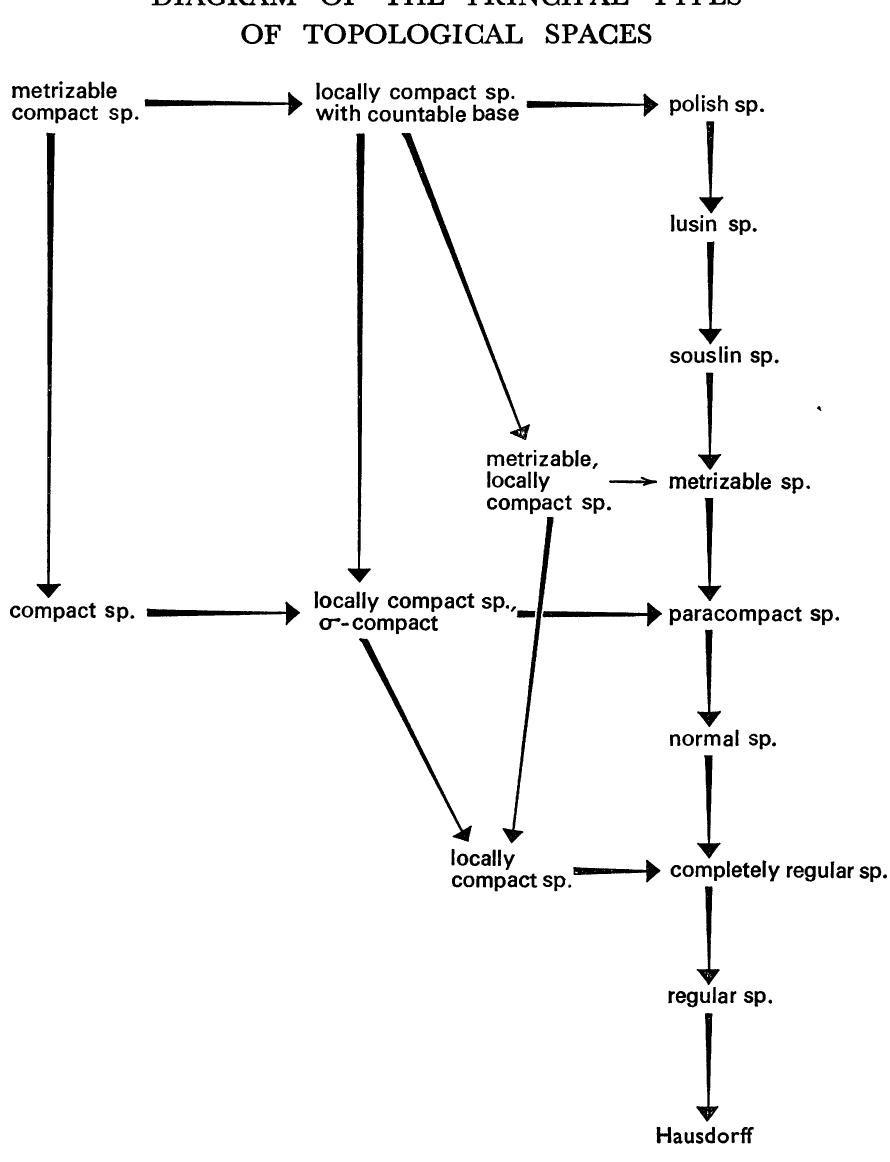
\includegraphics[keepaspectratio]{images/part002_2eb706e7.jpg}}

